%%%%%%%%%%%%%%%%%%%%%%%%%%%%%%%%%%%%%%%%%
% Journal Article
% LaTeX Template
% Version 1.4 (15/5/16)
%
% This template has been downloaded from:
% http://www.LaTeXTemplates.com
%
% Original author:
% Frits Wenneker (http://www.howtotex.com) with extensive modifications by
% Vel (vel@LaTeXTemplates.com)
%
% License:
% CC BY-NC-SA 3.0 (http://creativecommons.org/licenses/by-nc-sa/3.0/)
%
%%%%%%%%%%%%%%%%%%%%%%%%%%%%%%%%%%%%%%%%%

%----------------------------------------------------------------------------------------
%	PACKAGES AND OTHER DOCUMENT CONFIGURATIONS
%----------------------------------------------------------------------------------------

\documentclass[twoside,twocolumn]{article}

\usepackage{blindtext} % Package to generate dummy text throughout this template 

\usepackage[sc]{mathpazo} % Use the Palatino font
\usepackage[T1]{fontenc} % Use 8-bit encoding that has 256 glyphs
\linespread{1.05} % Line spacing - Palatino needs more space between lines
\usepackage{microtype} % Slightly tweak font spacing for aesthetics

\usepackage[english]{babel} % Language hyphenation and typographical rules

\usepackage[hmarginratio=1:1,top=32mm,columnsep=20pt]{geometry} % Document margins
\usepackage[hang, small,labelfont=bf,up,textfont=it,up]{caption} % Custom captions under/above floats in tables or figures
\usepackage{booktabs} % Horizontal rules in tables

\usepackage{lettrine} % The lettrine is the first enlarged letter at the beginning of the text

\usepackage{enumitem} % Customized lists
\setlist[itemize]{noitemsep} % Make itemize lists more compact

\usepackage{abstract} % Allows abstract customization
\renewcommand{\abstractnamefont}{\normalfont\bfseries} % Set the "Abstract" text to bold
\renewcommand{\abstracttextfont}{\normalfont\small\itshape} % Set the abstract itself to small italic text

\usepackage{titlesec} % Allows customization of titles
\renewcommand\thesection{\Roman{section}} % Roman numerals for the sections
\renewcommand\thesubsection{\roman{subsection}} % roman numerals for subsections
\titleformat{\section}[block]{\large\scshape\centering}{\thesection.}{1em}{} % Change the look of the section titles
\titleformat{\subsection}[block]{\large}{\thesubsection.}{1em}{} % Change the look of the section titles

\usepackage{fancyhdr} % Headers and footers
\pagestyle{fancy} % All pages have headers and footers
\fancyhead{} % Blank out the default header
\fancyfoot{} % Blank out the default footer
%\fancyhead[C]{Running title $\bullet$ May 2016 $\bullet$ Vol. XXI, No. 1} % Custom header text
\fancyfoot[RO,LE]{\thepage} % Custom footer text

\usepackage{titling} % Customizing the title section

\usepackage{hyperref} % For hyperlinks in the PDF

\usepackage{graphicx}
\usepackage{mathtools}
\usepackage{listings}
%\usepackage{epstopdf}

%----------------------------------------------------------------------------------------
%	TITLE SECTION
%----------------------------------------------------------------------------------------

\setlength{\droptitle}{-4\baselineskip} % Move the title up

\pretitle{\begin{center}\Huge\bfseries} % Article title formatting
\posttitle{\end{center}} % Article title closing formatting
\title{Explaining Hopcroft, Tarjan, Gutwenger, and Mutzel's SPQR Decomposition Algorithm} % Article title
\author{%
\textsc{Shoichiro Yamanishi}\\[1ex] % Your name
\normalsize \\ % Your institution
\normalsize \href{mailto:yamanishi72@gmail.com}{yamanishi72@gmail.com} % Your email address
%\and % Uncomment if 2 authors are required, duplicate these 4 lines if more
%\textsc{Jane Smith}\thanks{Corresponding author} \\[1ex] % Second author's name
%\normalsize University of Utah \\ % Second author's institution
%\normalsize \href{mailto:jane@smith.com}{jane@smith.com} % Second author's email address
}
\date{\today} % Leave empty to omit a date
\renewcommand{\maketitlehookd}{%
\begin{abstract}
The DFS based SPQR decomposition algorithm is explained.
Role of TSTACK is explained.
A simple case where the input graph does not have tree arc branches is explained  as a sweeping algorithm. 
The simple case is expanded to the general case with tree arc branches and role of TSTACK with EOS is explained.
Reason for the correction to $\phi$ calculation and the dynamic update of $HIGHPT(v)$ are given.
Some implementation subtleties are explained.

\noindent 
%\blindtext % Dummy abstract text - replace \blindtext with your abstract text
\end{abstract}
}

%----------------------------------------------------------------------------------------

\begin{document}

% Print the title
\maketitle

%----------------------------------------------------------------------------------------
%	ARTICLE CONTENTS
%----------------------------------------------------------------------------------------

\section{Overview}
A linear time SPQR decomposition algorithm using DFS was first presented
by Hopcroft \& Tarjan \cite{HT73}, and later it was corrected by Gutwenger \& Mutzel
\cite{GM01}.
The algorithm consists of 3 DFS explorations and some auxiliary subroutines.
\cite{GM01} isolates and clarifies the core of the algorithm called
{\it check for type-2 pairs}, or denoted by {\ttfamily Type2()} and {\it check for type-1 pair }, or
{\ttfamily Type1()},  as subroutines to the 3rd DFS called {\ttfamily PathSearch()}.
Even after the clarification made by \cite{GM01}, it seems difficult to the author
to understand the implementation of the algorithm presented in those papers.
This article attempts to fill the gap between the literature and
the implementation by explaining some key ideas with some examples.
This article also clarifies some ambiguities on some parts of the algorithm
that are not well explained in either of the papers above.
It is strongly recommended the readers read \cite{HT73} up to the proof of {\ttfamily Lemma 17},
 and \cite{GM01}.
Is is also recommended to read some other literature about the SPQR
 decompositon to familiarise ourselves with basic concepts and terminology
 such as virtual edges and skeleton.


%------------------------------------------------

\section{Restriction to Simple Graphs}

Here in this article only simple biconnected graphs are considered.
Restricting the input graphs to be simple simplifies the DFS explorations
and handling of split components when new components are found in
{\ttfamily Type1()} and {\ttfamily Type2()} by eliminating the need to handle 2-cycles.
This restriction is not severe, as we can handle multi-graphs by extra
pre- and post-processing. We temporarily remove self-loops and bundle
multi-edges into single edges before running the algorithm, and after the
 SPQR decomposition, the self-loops are restored, and additional P-nodes are
further added for those multi-edges bundled.

With this restriction, the only places in the algorithm where multi-edges
occur are in the split components of 3-bonds (minimal P-nodes) during
{\ttfamily PathSearch()}, and in the split component of P-nodes during and after the
merger of consecutive 3-bonds into a maximal bonds in Algorithm 2 of \cite{GM01}.
The 3rd DFS, called {\ttfamily PathSearch()} is a destructive process where at each step
up to 3 minimal split components can be separated from the input graph at
a specific separation pair $\{a,b\}$, and the input graph denoted by $G_c$ in \cite{GM01}
will be reduced and will become a new skeleton with a virtual edge $\{a,b\}$.
The simplicity of the input graph will remain invariant through the process
of {\ttfamily PathSearch()}, which  makes the implementation simpler.

If a multi-graph without self-loops were given to the algorithm described as in
\cite{GM01}, the separation pairs found in {\ttfamily Type1()} and {\ttfamily Type2()} will no longer be
minimal. Also, a special care will have to be taken if the frond that ends
a path is a multi-edge, in which case the lowest node (start of the path),
and the highest node of the path form a separation pair candidate in {\ttfamily TSTACK}
 as the first element pushed, and then it could be falsely considered a
separation pair when the lowest node of the path is visited in a
post-traversal.
With all those extra complications, the author thinks the best way to
handle biconnected multi-graphs is to temporarily remove multi-edges and
self-loops before running the algorithm.

\section{Roles Of Virtual Edges}
A virtual edge has three roles.
\begin{itemize}
\item Specifies the location of the split pair in the split components.
\item Keeps $G_c$ biconnected. $G_c$ is the graph explored by {\ttfamily PathSearch()}.
\item Makes the skeleton tri-connected in the R nodes.
\end{itemize}


\section{Key to Understanding the Algorithm: Type 1 and Type 2 separation pairs}

The problem of finding the triconnected components and thus finding the
SPQR-tree of a simple biconnected graph is reduced to finding the type-1 and
type-2 pairs as {\bf Lemma 3} in \cite{GM01} states (Fig. \ref{fig:fig1} and \ref{fig:fig2}).

\begin{figure}[!htb]
\centering
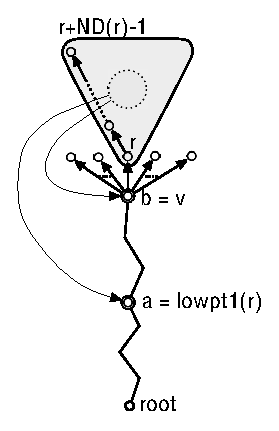
\includegraphics[scale=1.0]{spqr_fig1.eps}
\caption{Type 1 Separation Pair}
\label{fig:fig1}
\end{figure}

\begin{figure}[!htb]
\centering
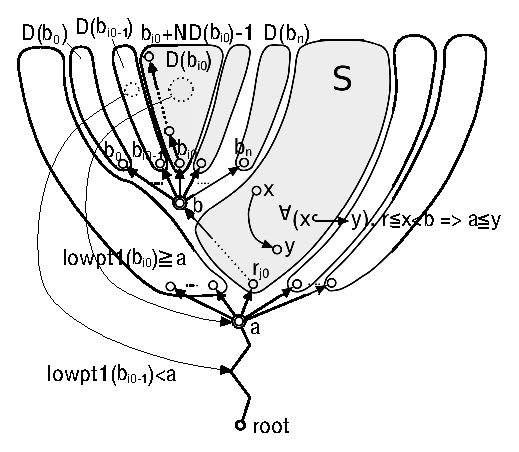
\includegraphics[scale=0.9]{spqr_fig2.eps}
\caption{Type 2 Separation Pair}
\label{fig:fig2}
\end{figure}

This is the key observation that leads to the algorithm found in \cite{HT73}.
We could develop a divide-and-conquer type algorithm at each split pair found,
 and applying it recursively to the (not necessarily minimal) split components
 after each split.
The algorithm in \cite{HT73} and \cite{GM01} takes a clever iterative and recursive
approach that runs in $O(|V|+|E|)$ time utilising DFS.
It is iterative in a sense that the algorithm scans for a minimal split
component
 along a path in the palm-tree in the descending order of node number
assigned, and it is recursive on the paths found at the new frond or a tree
branch.

Finding the minimal split components iteratively is achieved by a clever
placement of {\ttfamily Type2()} and {\ttfamily Type1()} in {\ttfamily PathSearch()}.
Finding them recursively is achieved by a clever use of node numbering and
the {\ttfamily EOS} markers on {\ttfamily TSTACK} for each recursion.

In the following we first deal with the simple case without recursion and
we study the core of the algorithm around the use of the three values on
{\ttfamily TSTACK} for the type-2 pairs.
Then we expand the discussion to the recursive case by explaining
the role of the {\ttfamily EOS} markers and the modification of {\ttfamily TSTACK}
in the transition to the new path in {\ttfamily PathSearch()}.
Before walking through a simple case without recursion, we will briefly review
{\ttfamily TSTACK} first.




\section{Role of TSTACK}

We will review the meaning of $h$, $a$, \& $b$, and some notations relevant to
them with Fig. \ref{fig:fig2}.  Hereafter we will use node $a$ to mean the node number as
 well as the identity of the node interchangeably.
Node $a$ and node $b$ in an element of {\ttfamily TSTACK} are the lower and higher nodes of a
type-2 separation pair candidate.
Node $b$ must be on the left most path from a child $r_{j0}$ of
node $a$. In \cite{HT73} \& \cite{GM01}, such a node like $b$ is called the first descendent of
$r_{j0}$,  and it is denoted by $r_{j0}\xrightarrow* b$. In the same way, $h$ is on the left most
path from
 a child $b_{i0}$ of $b$. The node $h$ is also the highest descendant of $b_{i0}$.
The value $h$ is $b_{i0} + ND(b_{i0}) - 1$.
The triplet ($h$, $a$, $b$) is enough to describe the corresponding minimal
split components.  The node induced by the split components is given by
$D(b_{i0}) \cup\cdots\cup D(b_n) \cup S \cup \{a,b\}$ according to the proof of
{\bf Lemma 17} in \cite{HT73}. In the range of node numbers, it can be expressed as
$[r_{j0}, h]$ and $a$.
In the algorithm it can be simply expressed as $[a,h]$, and the condition
 to find the edges for the separation class is given by $a \leq x \leq h \wedge a \leq y \leq h$ in
{\ttfamily Type2()}. This is because the nodes in $D(r_j), j < j0$, i.e., $r_j$
is a child of a to the left of $r_j$, have higher numbers than $h$, and also
from the way DFS is performed, and from the order in which the visited edge
is pushed onto {\ttfamily ESTACK}, the nodes $r_j, j > j0$, i.e., to the right of $r_{j0}$
in the siblings of $a$, have yet been explored, and hence the edges to the right
 of $S$ and $\{a ,r_j\}$ are not yet pushed onto {\ttfamily ESTACK}. This is the reason why the
range $a \leq x \leq h \wedge a \leq y \leq h$ works to identify the edges in the split component.

\section{DFS Walk 1: Tree without Branches}

First, we deal with the case of a simple tree where tree arcs form a single
straight path with no branches, which does not involve {\ttfamily EOS} on {\ttfamily TSTACK},
and in which $h$ always coincides with $b$ on {\ttfamily TSTACK}.
This shows the basic idea of the sweeping algorithm of the type 2 part of {\ttfamily PathSearch()}.
See Fig. \ref{fig:fig3}.

\begin{figure}[!htb]
\centering
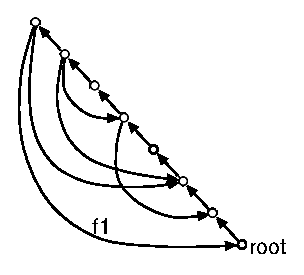
\includegraphics[scale=1.0]{spqr_fig3.eps}
\caption{$G_c$ without tree branches}
\label{fig:fig3}
\end{figure}


It is easy to see the following according to {\ttfamily Algorithm 4: PathSearch()} of
\cite{GM01}.

\begin{itemize}
\item All the tree arcs from the root and the first frond $f1$ back to the root
together form the first path.
\item The second path onwards each consists of a single frond.
\end{itemize}

Whenever a frond that starts a path, (i.e., any frond other than $f1$) is visited,
 {\ttfamily TSTACK} is updated.
If there is no element removed from {\ttfamily TSTACK}, which basically means if there is
no frond criss-crossing the current frond, we will put ($v$, $w$, $v$) on top of the
current stack (Fig. \ref{fig:fig4}).
$\{w,v\}$ is a separation pair candidate with the corresponding separation class with edges
 incident to the vertices on the path from $v$ to $w$. This will be tested when
DFS exploration comes back to $w$, if it is still on {\ttfamily TSTACK}.
On the other hand, if there are some elements removed from {\ttfamily TSTACK},
this means there are some fronds criss-crossing $\{w,v\}$ (Fig. \ref{fig:fig5}).
Because of the presence
of $v$ coming out of those $\{a_i,b_i\}, 0 \leq i \leq k$ pairs, those can no longer be candidates
for a separation pair. A possibility is $w$ as the lower node, and the highest
(outer most) $b_{k}$. In this case, the corresponding split component will be
specified by the highest (outer most) $h_{k}$, which coincides with $b_{k}$.
Conceptually, those removed fronds on {\ttfamily TSTACK} and the frond $\{v,w\}$ are merged
into a new frond as a split pair candidate on top of {\ttfamily TSTACK}.
This is what happens in the bottom half of {\ttfamily PathSearch()} in \cite{GM01}, where
a frond $(v \hookrightarrow w)$ is handled.

\begin{figure}[!htb]
\centering
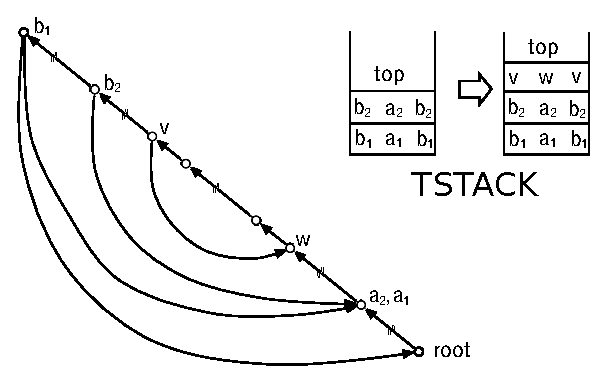
\includegraphics[scale=0.7]{spqr_fig4.eps}
\caption{$v \hookrightarrow w$ not crossing others}
\label{fig:fig4}
\end{figure}

\begin{figure}[!htb]
\centering
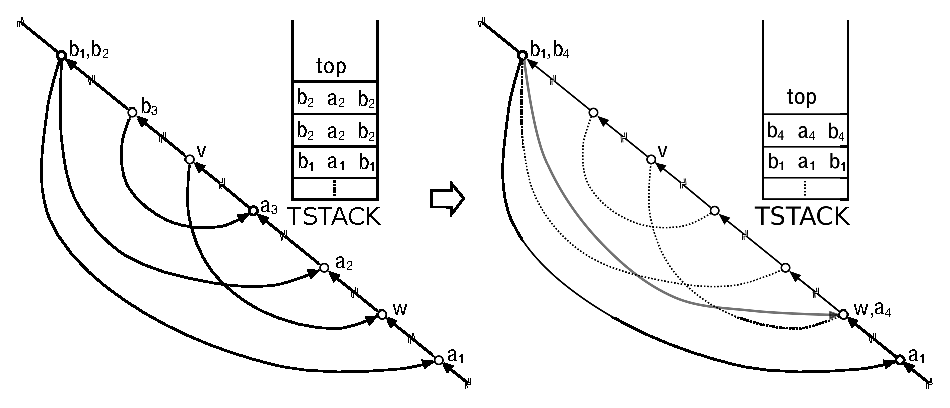
\includegraphics[scale=0.5]{spqr_fig5.eps}
\caption{$v \hookrightarrow w$ crossing others}
\label{fig:fig5}
\end{figure}

One might wonder if there is a case where $a_i$ are above or coincide with $v$,
but we can show such a case can not happen.
Suppose there is a pair $\{a_j,b_j\}$ such that $a_j$ is above or coincides with $v$
 on top {\ttfamily TSTACK}. Then such a pair would have been a proper separation pair
found in {\ttfamily Type2()} when $(a_j \rightarrow r)$, where $r$ is the child of $a_j$
 on the tree arc, was examined in {\ttfamily PathSearch()}, and such a pair would have
 been removed in it. A contradiction.
 Please note that if $a_j$ coincides with $v$, then
 the tree arc $(v \rightarrow r)$ has been visited before the frond $(v \hookrightarrow w)$ from the way
 incidence list for each node is created by the $\phi$ value for each edge (Fig. \ref{fig:fig6}).
  In general, when the DFS is leaving
a node $v$, then {\ttfamily TSTACK} does not contain any element whose $a$ is greater (higher)
than $v$ from the top down to {\ttfamily EOS} marker, which will be explained in the next
section.

\begin{figure}[!htb]
\centering
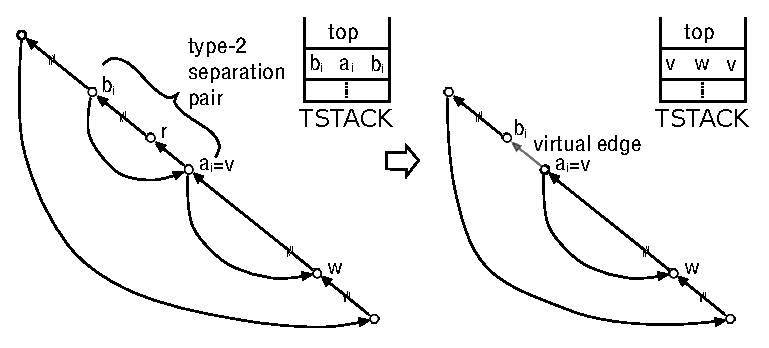
\includegraphics[scale=0.6]{spqr_fig6.eps}
\caption{$a_i$ \& $b_i$ evaluated before $(v \hookrightarrow w)$ is processed}
\label{fig:fig6}
\end{figure}

There is one thing we have to take care after {\ttfamily TSTACK} is updated as above, which
conceptually means merging the fronds into one. After the merger, the
information about the arrivals of the fronds at $a_i$ will be lost from {\ttfamily TSTACK}.
This will cause a false finding of a separation pair as shown in Fig. \ref{fig:fig7}.
In Fig. \ref{fig:fig7}, when the frond $(v \hookrightarrow w)$ is processed, two elements on {\ttfamily TSTACK},
 ($b_2$, $a_2$, $b_2$) and ($b_1$, $a_1$, $b_1$) are merged to ($b_1$, $w$, $b_1$), later
when $a_4$ is being visited, it falsely finds ($b_3$, $a_4$,  $b_3$) on {\ttfamily TSTACK} as
a separation pair, but it is not due to the frond $(b_2 \hookrightarrow a_2)$,
which has been lost from {\ttfamily TSTACK}.

\begin{figure}[!htb]
\centering
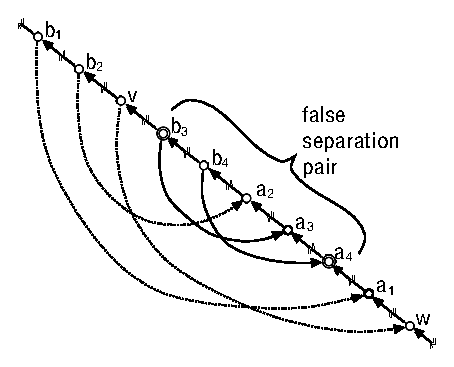
\includegraphics[scale=1.0]{spqr_fig7.eps}
\caption{Avoid false detection of separation pairs}
\label{fig:fig7}
\end{figure}

To avoid finding such a false separation pair, we have to remove invalid fronds
from {\ttfamily TSTACK}, and it is done at the end of a visit to $(v \rightarrow w)$ in {\ttfamily PathSearch()}.
It removes elements from {\ttfamily TSTACK} whose $h$ values are less than the current
node $v$. For example when the DFS exploration is at the end of a visit to
$\{a_1,r_1\}$ along the path, $a_1$'s high point is found to be $b_1$.
All the elements whose $h$ value (and hence $b$ value) is less than the high point
 are removed. This prevents detection of false separation pairs.
For the case in Fig. \ref{fig:fig7}, at the end of the visit to $a_2$, the high point of $a_2$
is found to be $b_2$, and the element ($b_3$, $a_4$, $b_3$) is removed from {\ttfamily TSTACK}.

The algorithm proceeds in this way from the higher nodes down toward the tree
 root iteratively. This can be considered a sweeping algorithm.
Along the exploration, at a node $v$, if there is an element on {\ttfamily TSTACK} whose a
conincides with $v$, then this means there is no frond coming in or going out
between $a$ and $b$ (not including $a$ and $b$), and $\{a,b\}$ form a separation pair with
 all the edges between $\{a,b\}$ inclusive. See Fig. \ref{fig:fig8}.

\begin{figure}[!htb]
\centering
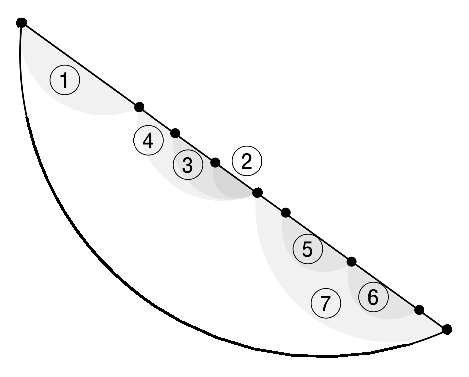
\includegraphics[scale=1.0]{spqr_fig8.eps}
\caption{Order in which type-2 pairs are detected}
\label{fig:fig8}
\end{figure}


Also we are sure that the split component found by ($h$, $a$, $b$) is minimal from
the way the fronds have been explored. If some elements on {\ttfamily TSTACK} share the
same $a$, then the element with the closest $b$ is always on top, and if some
elements on {\ttfamily TSTACK} share the same $b$, then the element with the closest $a$ is
always on top.

After the separation class is removed, $\{a,b\}$ will be inserted to $G_c$ as a
virtual edge, the current top on {\ttfamily TSTACK} is removed, and
{\ttfamily Type2()} tries to find another separation pair with the same $a$
(=$v$) if there is any on {\ttfamily TSTACK}. See 2, 3, 4 in Fig. \ref{fig:fig8}.
If not, then DFS exploration moves on to the next node below $v$.
This sweeping continues until DFS exploration hits the root node,
by which time all the separation pairs will have been found.


\section{Handling Type 1 Cases}
The check for a type 1 separation pair is done after the checks for type 2
 pairs are done, and the check is done only once.
The reason for testing type 2 first, possibly multiple times, and then testing
 type 1 at most once, is as follows.
At each current node $v$, $G_c$ must be tested for Type 2 first to ensure
the split component found is minimal, i.e., the split component should not
 be able to be split into two separation classes further by another separation pair
 in the node set induced by the separation class.
Fig. \ref{fig:fig9} illustrates this. Suppose the current node for the DFS exploration is $v$,
 we see two separation pairs: $\{v, b\}$ as Type 2, and $\{v, lowpt1(v)\}$ as Type 1.
If we test for Type 1 first, the separation class will contain another split
pair $\{v,b\}$, which is against minimality.
The minimality among the multiple split components found in {\ttfamily Type2()}
are minimal due to the way {\ttfamily TSTACK} is constructed, updated, and tested as
shown above.
Also, we don't have to test for Type 1 more than once.
There can be another separation class with the same separation pair, but those will be found when DFS exploration comes 
back to $v$ from a different neighbour (Fig. \ref{fig:fig10}).

\begin{figure}[!htb]
\centering
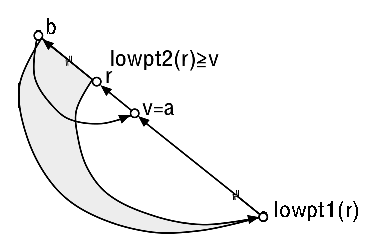
\includegraphics[scale=1.0]{spqr_fig9.eps}
\caption{Detection of Type 1 pair}
\label{fig:fig9}
\end{figure}

\begin{figure}[!htb]
\centering
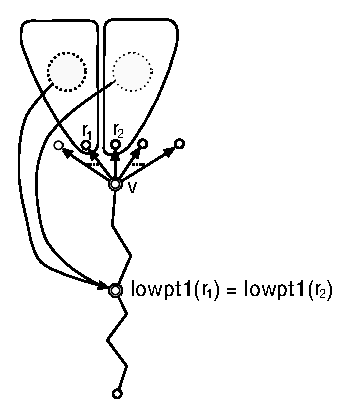
\includegraphics[scale=1.0]{spqr_fig10.eps}
\caption{Two split components with the same Type 1 pair}
\label{fig:fig10}
\end{figure}


\section{Handling Triangles (Minimal S-type separation class}
Triangles are handled as a special case in both {\ttfamily Type2()} and {\ttfamily Type1()}.
{\ttfamily Type2()} deals with $v \rightarrow w \rightarrow x$, while {\ttfamily Type1} deals with $v \rightarrow w \hookrightarrow x$.
The former can't be handled by {\ttfamily TSTACK}, and therefore it is detected
by an explicit condition $deg(w)=2 \wedge firstChild(w) > w$ in {\ttfamily Type2()}
as shown in Fig. \ref{fig:fig11}.
The latter is detected as a minimal case for Type 1, which is
$lowpt1(w) < v \wedge lowpt2(w) \geq v$ as shown in Fig. \ref{fig:fig12}.


\begin{figure}[!htb]
\centering
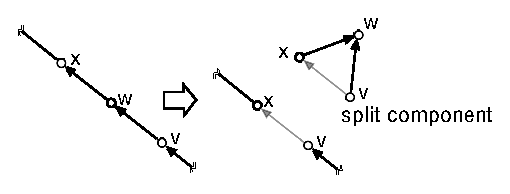
\includegraphics[scale=1.0]{spqr_fig11.eps}
\caption{Type 2 triangle}
\label{fig:fig11}
\end{figure}

\begin{figure}[!htb]
\centering
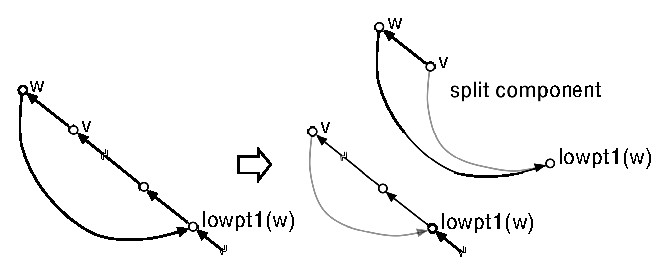
\includegraphics[scale=0.8]{spqr_fig12.eps}
\caption{Type 1 triangle}
\label{fig:fig12}
\end{figure}

\section{$\phi$ Value and Order of Incidence Edges of Each Node}

\cite{GM01} corrects the calculation of $\phi$ value of each edge as follows.
\[
\phi(e) = \left\{ \begin{array}{lcl}
3lowpt1(w) & \mbox{if} & e = v \rightarrow w \wedge lowpt2(w) < v \\
3w + 1 & \mbox{if} & e = v \hookrightarrow w \\
3lowpt1(w) + 2 & \mbox{if} & e = v \rightarrow w \wedge lowpt2(w) \geq v
\end{array}\right.
\]

\cite{GM01} states reason for the correction as to identify all multiple edges,
but it is not clear why this correction is needed. Basically this is relevant
to {\ttfamily Type1()} and the order in which the edges are pushed to
{\ttfamily ESTACK}. Suppose {\ttfamily PathSearch()} is visiting $v$ from $w_{i0}$ in the post traversal as in Fig. \ref{fig:fig13}, and it
has detected a Type 1 separation pair $\{ v, lowpt1(w_{i0})\}$, in which case
$lowpt2(w_{i0}) \geq v$. Also suppose there is a frond $(v \hookrightarrow lowpt1(w_{i0}))$.
We must have visited it before visiting the tree arc $(v \rightarrow w_{i0})$, so that the it
is the first edge pushed to {\ttfamily ESTACK} and hence the last one popped in the following if clause after the while loop
 in {\ttfamily Type1()}.
\begin{ttfamily}
\begin{lstlisting}
 ESTACK.top() = (v,lowpt1(w)) then
\end{lstlisting}
\end{ttfamily}

The $\phi$ calculation proposed in \cite{GM01} ensures this order, but the one
proposed in \cite{HT73} does not.

\begin{figure}[!htb]
\centering
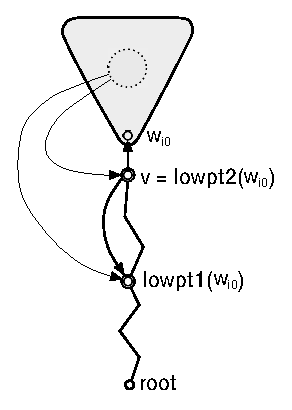
\includegraphics[scale=1.0]{spqr_fig13.eps}
\caption{An edge between a type-1 separation pair}
\label{fig:fig13}
\end{figure}

\section{DFS Walk 2: General Case with Tree Branches and EOS}
Finally, we will expand the discussion to the general case for the palm-trees
with tree branches.
First, imagine there is a branch from a node v as shown in Fig. \ref{fig:fig14}.
Here, the tree arc $(v \rightarrow w)$ marks the start of a new path that follows
 the left-most tree arcs and ends with the deepest frond, whose destination
 node corresponds to $lowpt1(w)$. {\ttfamily TSTACK} is updated according to {\ttfamily PathSearch()}.
 The basic idea is the same as for the single path case, and the path
 $v \rightarrow w \xrightarrow* h \hookrightarrow lowpt1(w)$ can be considered a frond from $v$ to $lowpt1(w)$.
 The criss-crossing fronds with the current ones are
 removed from {\ttfamily TSTACK}, merged with the current one, and a single new element is
pushed to {\ttfamily TSTACK}. In Fig. \ref{fig:fig14}, the two elements ($b_1$, $a_1$, $b_1$) and ($b_2$, $a_2$, $b_2$) 
are removed from {\ttfamily TSTACK}
and a new element ($b_2$, $lowpt1(w)$, $b_2$) is pushed.
 The difference is that now $h$ is different from $b$.
Node $b$ is at the branching node on the current path, which is $v$,
and node $h$ is the highest possible node along the left-most path from node $w$.
Node $a$ is lowest reachable from $w$, which is $lowpt1(w)$.
Then the modification of {\ttfamily TSTACK} for the current path is done, and an {\ttfamily EOS} marker is pushed on to {\ttfamily TSTACK}
to prepare for the recursive processing for the new path that starts with $(v \rightarrow w)$.

Here we observe the following two invariants on the current path.
\begin{itemize}
\item The conceptual (merged) fronds formed by $(a \hookrightarrow b)$ on {\ttfamily TSTACK} are not criss crossing.
\item The nodes for $b$ are always on the current path.
\end{itemize}

\begin{figure}[!htb]
\centering
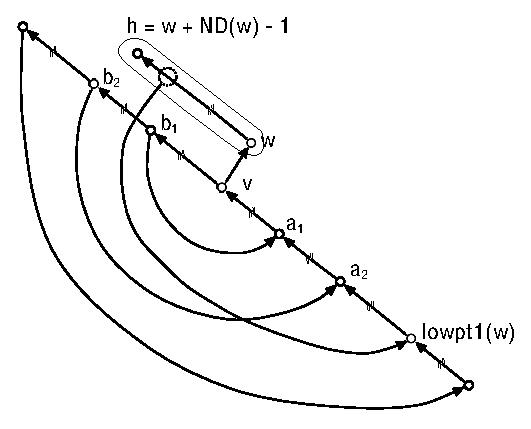
\includegraphics[scale=1.0]{spqr_fig14.eps}
\caption{New path from $v$}
\label{fig:fig14}
\end{figure}


We also observe the nodes for $a$ on {\ttfamily TSTACK} can no longer be on the current path.
{\bf Lemma 3} in \cite{GM01} requries $b$ to be on the left-most path from a child of node $a$.
The following explains how the algorithm handles this condition properly.
See Fig. \ref{fig:fig15}. In this case the current path starts from node $c$ along the thicker line. At some point
at a tree branch, {\ttfamily TSTACK} gets an element ($h$, $v$, $lowpt1(w)$), and $lowpt1(w)$ is located down on an earlier path.
If the DFS visits $c$ in the post traversal, it checks if $c$ coincides with node $a$ on top of {\ttfamily TSTACK}.
If it does (Fig. \ref{fig:fig15} b), then the top of {\ttfamily TSTACK} will be a separation pair. If it does not (Fig. \ref{fig:fig15} a),
then all the elements for the current paths including {\ttfamily EOS} marker are removed from {\ttfamily TSTACK} at the end of the visit.

To avoid false detection of a separation pair, {\ttfamily PathSearch()} removes elements from {\ttfamily TSTACK} at the end of a visit
to a tree arc just like the case of a simple path described before.
All the elements whose $h$ is less than {\ttfamily HIGHPT(v)} are removed. The reason why $h$ is used instead of $b$ is that
unlike for the case of a simple path, $b$ and $h$ can have different values, and there can be multiple elements
with different $h$ value but with the same $b$ value. Fig. \ref{fig:fig16} is such a case.
This is equivalent to avoiding finding false separation pair to the left of $D(b_{i0})$ in Fig. \ref{fig:fig2}.

Overall, whenever the DFS enters a new tree arc that starts a path, update the elements on {\ttfamily TSTACK} as shown in {\ttfamily PathSearch()}
in \cite{GM01}, place {\ttfamily EOS} on top to temporarily suspend the processing on the current path, then move on to the newly discovered path.
On the new path the DFS tries to find separation pairs along the new path, and also when the DFS comes back to the node where the new path has started, e.g., $c$ in Fig. \ref{fig:fig15} (b), if there is an element on TSTACK whose $a$ coincides with the node, then the separation pair and the split components are processed. This is done recursively whenever a new path is found along the DFS exploration.

\begin{figure}[!htb]
\centering
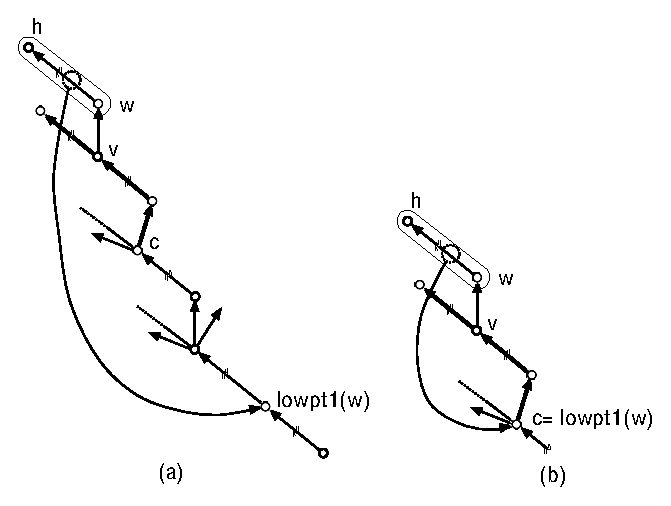
\includegraphics[scale=0.7]{spqr_fig15.eps}
\caption{$a$ not necessarily on the current path}
\label{fig:fig15}
\end{figure}


There is a subtle point in updating the {\ttfamily TSTACK} in the beginning of the tree arc that starts a path.
If some elements are removed from {\ttfamily TSTACK}, then the outer-most $b$ will be used for the new element to be pushed.
The outer-most $b$ coincides with $b$ in the last element removed.
However, we can't simply use $h$ in the last element. The reason is that the elements from fronds and elements
from tree arcs that start new paths that share the same $b$ are intertwined on {\ttfamily TSTACK}.
See Fig. \ref{fig:fig17}. In this case the element from the frond $(v \hookrightarrow w_1)$ is at the bottom. Later when the frond
$(x \hookrightarrow y)$ is processed those three elements are removed from {\ttfamily TSTACK} and a new h is not from the last element
removed due to the presence of the element from fronds.

One might wonder if a similar treatment is necessary when elements of {\ttfamily TSTACK} whose $h$ are less than {\ttfamily HIGHPT(v)} are
removed. For example if there is a frond in Fig. \ref{fig:fig16} such that $(b \hookrightarrow a_0), a_0 < a_1$. In this case there can be
($b$, $a_0$, $b$) below ($h_1$, $a_1$, $b$) on {\ttfamily TSTACK} when the DFS is visiting $v$, and the removal stops when it sees ($h_1$, $a_1$, $b$), 
and ($b$, $a_0$, $b$)  will go unremoved. However this might cause a false detection of separation pair. If ($b$, $a_0$, $b$) is still on {\ttfamily TSTACK}
when the DFS is visiting $a_1$, then $HIGHPT(a_1) > b_1$, and   ($b$, $a_0$, $b$) will be removed there before the DFS reaches $a_0$ in the post traversal.

\begin{figure}[!htb]
\centering
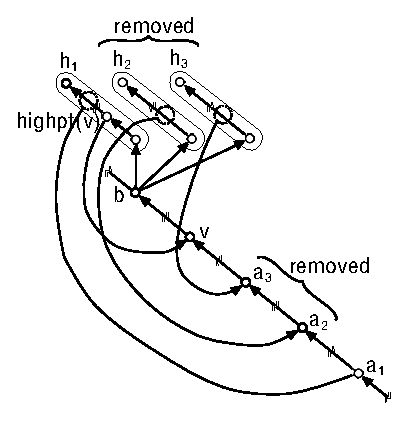
\includegraphics[scale=1.0]{spqr_fig16.eps}
\caption{Removing invalid elements from TSTACK}
\label{fig:fig16}
\end{figure}

\begin{figure}[!htb]
\centering
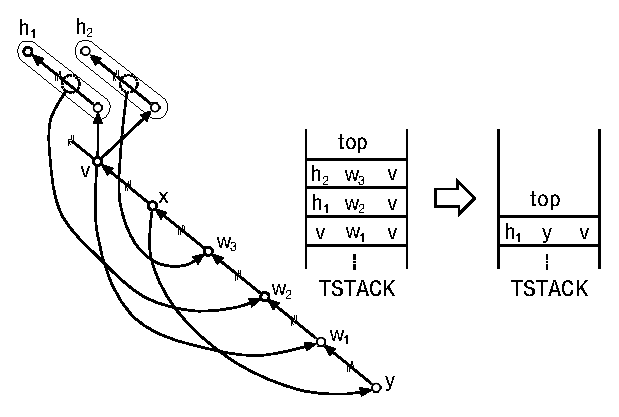
\includegraphics[scale=0.7]{spqr_fig17.eps}
\caption{Order of elements that share the same $b$ on TSTACK}
\label{fig:fig17}
\end{figure}

\section{Reason Why Dynamic Updates Are Needed for HIGHPT}

\cite{GM01} states the need for updates of {\ttfamily HIGHPT} for each node on-the-fly, but
it does not state the reason. Fig. \ref{fig:fig18} explains this in relation to
invalid elements removal on {\ttfamily TSTACK} at the end of each visit to $v$ explained
above. In Fig. \ref{fig:fig18} (a), node $a'$ is the current node being visited, and it finds
($h_1$,$a_1$, $b_1$) on top of the stack. Supposed {\ttfamily HIGHPT($a'$) = $b'$}.  In Fig. \ref{fig:fig18} (a),
the subgraph from $b_1$-$b'$-$h'$ still remains in $G_c$ and hence ($h_1$, $a_1$, $b_1$) has
to be removed. However, there are some cases in which by the time DFS visits
node $a'$ on its way back (post-traversal), the subgraph induced by $b_1$, $b'$ and $h'$
has been removed from $G_c$ as separation classes. In this case ($h_1$, $a_1$, $b_1$) is a valid
separation pair candidate and it should be kept on {\ttfamily TSTACK}. Since wether
or not to remove ($h_1$, $a_1$, $b_1$) is detemined by {\ttfamily HIGHPT($a'$)}, keeping it up-to-date
during the DFS traversal is necessary.

\begin{figure}[!htb]
\centering
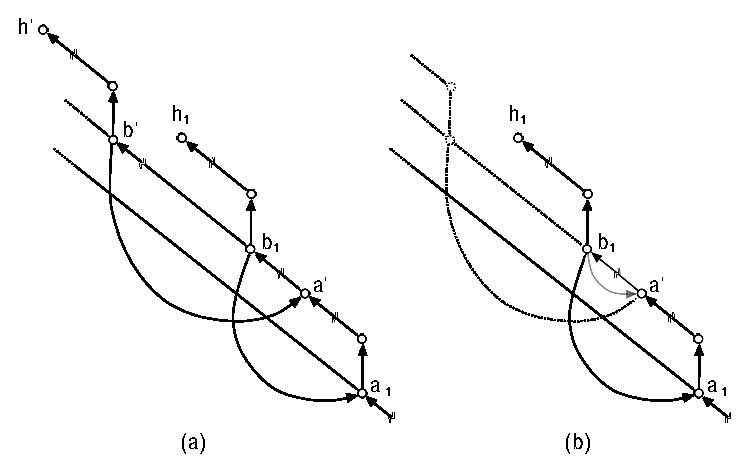
\includegraphics[scale=0.7]{spqr_fig18.eps}
\caption{Need to update HIGHPT}
\label{fig:fig18}
\end{figure}


%------------------------------------------------
%----------------------------------------------------------------------------------------
%	REFERENCE LIST
%----------------------------------------------------------------------------------------

\begin{thebibliography}{99} % Bibliography - this is intentionally simple in this template

\bibitem[HT73]{HT73}
Hopcroft, J.E. and Tarjan, R.E. (1973).
\newblock Dividing a graph into triconnected components
\newblock {\em SIAM J. Comput.}, 2(3):135-158.

\bibitem[GM01]{GM01}
Gutwenger, C. and Mutzel P. (2001).
\newblock A linear time implementation of SPQR-trees
\newblock {\em Proc. 8th International Symposium on Graph Drawing (GD2000)}, Lecture Notes in Computer Science 1984, Springer-Verlag, pp. 77-90
 
%\bibitem[SY16]{SY16}
%Yamanishi, S. (2016).
%\newblock Tarjan: Graph Decomposition and Planarization Library
%\newblock https://github.com/ToBeDecided
 

\end{thebibliography}

%----------------------------------------------------------------------------------------

\end{document}
